\documentclass{standalone}
\usepackage{pgfplots}
\pgfplotsset{compat=1.10}
\usetikzlibrary{patterns}
\usepackage{tkz-fct}
\usetikzlibrary{intersections}
\begin{document}

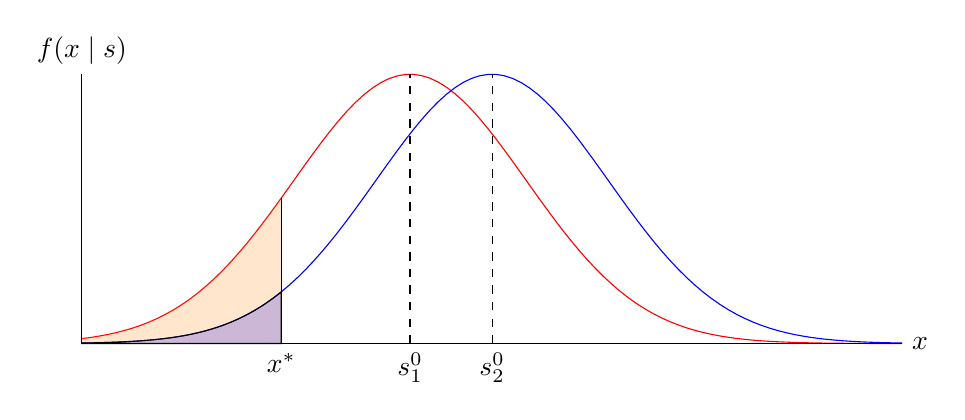
\begin{tikzpicture}[
declare function={ normal(\x,\u,\s) = 1/(\s*sqrt(2*pi))*exp(-pow((\x-\u),2)/(2*\s));
                 },
]

\begin{axis}[
  no markers, domain=-2:8, samples=100,
  axis lines*=left, 
  xlabel=$x$, ylabel=$f(x\mid s)$,
  every axis y label/.style={at={(ticklabel* cs:1)}, anchor=south,},
  every axis x label/.style={at=(current axis.right of origin),anchor=west},
  height=5cm, width=12cm,
  xtick=\empty, ytick=\empty,
  enlargelimits=false, clip=false, axis on top,
  grid = major
] % extend the axes a bit to the right and t
    						
\addplot[mark=none, red]  {normal(x,2,2)};
\addplot[mark=none, blue] {normal(x,3,2)};
\pgfmathsetmacro\meanone{normal(2,2,2)}
\pgfmathsetmacro\meantwo{normal(3,3,2)}
%mean
\draw[dashed] (axis cs:2,0) -- (axis cs:2,\meanone);
\draw[dashed] (axis cs:3,0) -- (axis cs:3,\meantwo);
\node[below] at (axis cs:2,0){$s^0_1$};
\node[below] at (axis cs:3,0){$s^0_2$};
%power 

\addplot+ [
    fill=orange,
    fill opacity=0.2,
    draw=none,
    domain=-2:0.43,
    stack plots=y
] {normal(x,2,2)} \closedcycle;
% alpha value
\pgfmathsetmacro\alphaval{normal(0.43,2,2)}
\draw[solid] (axis cs:0.43,0) -- (axis cs:0.43,\alphaval);
\node[below] at (axis cs:0.43,0){$x^*$};
\addplot+[mark=none, domain=-2:0.43, 
        fill=blue,
        fill opacity=0.2,
        area legend]  {normal(x,3,2)} \closedcycle; 
\end{axis}


\end{tikzpicture}

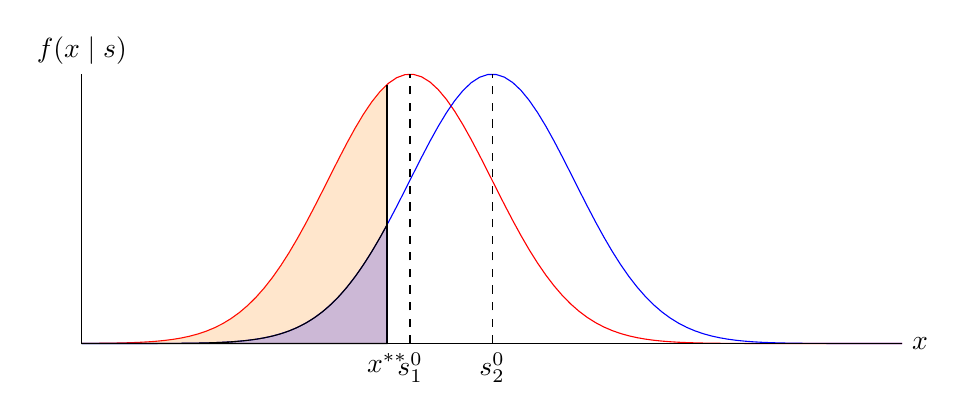
\begin{tikzpicture}[
declare function={ normal(\x,\u,\s) = 1/(\s*sqrt(2*pi))*exp(-pow((\x-\u),2)/(2*\s));
                 },
]

\begin{axis}[
  no markers, domain=-2:8, samples=100,
  axis lines*=left, 
  xlabel=$x$, ylabel=$f(x\mid s)$,
  every axis y label/.style={at={(ticklabel* cs:1)}, anchor=south,},
  every axis x label/.style={at=(current axis.right of origin),anchor=west},
  height=5cm, width=12cm,
  xtick=\empty, ytick=\empty,
  enlargelimits=false, clip=false, axis on top,
  grid = major
] % extend the axes a bit to the right and t
                
\addplot[mark=none, red]  {normal(x,2,1)};
\addplot[mark=none, blue] {normal(x,3,1)};
\pgfmathsetmacro\meanone{normal(2,2,1)}
\pgfmathsetmacro\meantwo{normal(3,3,1)}
%mean
\draw[dashed] (axis cs:2,0) -- (axis cs:2,\meanone);
\draw[dashed] (axis cs:3,0) -- (axis cs:3,\meantwo);
\node[below] at (axis cs:2,0){$s^0_1$};
\node[below] at (axis cs:3,0){$s^0_2$};
%power 
\addplot+ [
    fill=orange,
    fill opacity=0.2,
    draw=none,
    domain=-2:1.72,
    stack plots=y
] {normal(x,2,1)} \closedcycle;

% alpha value
\pgfmathsetmacro\alphaval{normal(1.72,2,1)}
\draw[solid] (axis cs:1.72,0) -- (axis cs:1.72,\alphaval);
\node[below] at (axis cs:1.72,0){$x^{**}$};
\addplot+[mark=none, domain=-2:1.72, 
        fill=blue,
        fill opacity=0.2,
        area legend]  {normal(x,3,1)} \closedcycle; 


\end{axis}


\end{tikzpicture}

\end{document}            